% -*- latex -*-
%%%%%%%%%%%%%%%%%%%%%%%%%%%%%%%%%%%%%%%%%%%%%%%%%%%%%%%%%%%%%%%%
%%%%%%%%%%%%%%%%%%%%%%%%%%%%%%%%%%%%%%%%%%%%%%%%%%%%%%%%%%%%%%%%
%%%%
%%%% This text file is part of the source of 
%%%% 'Parallel techniques'
%%%% by Ángel de Vicente, copyright 2019
%%%%
%%%% TO DO:
%%%%
%%%% basic-fortran.tex : basic fortran towards a first N-body implementation
%%%%
%%%%%%%%%%%%%%%%%%%%%%%%%%%%%%%%%%%%%%%%%%%%%%%%%%%%%%%%%%%%%%%%
%%%%%%%%%%%%%%%%%%%%%%%%%%%%%%%%%%%%%%%%%%%%%%%%%%%%%%%%%%%%%%%%

\Level 0 {Basic Fortran}
\label{sec:basic-fortran}

In this chapter we will just cover the basic concepts of Fortran. Fortran is a
complex language, so in this chapter we will only cover the surface of the
language, only the necessary minimum to be able to write a first implementation
of the N-body problem.

The following slides are taken from a 5-day intentive course on Fortran, given by the
University of Liverpool.

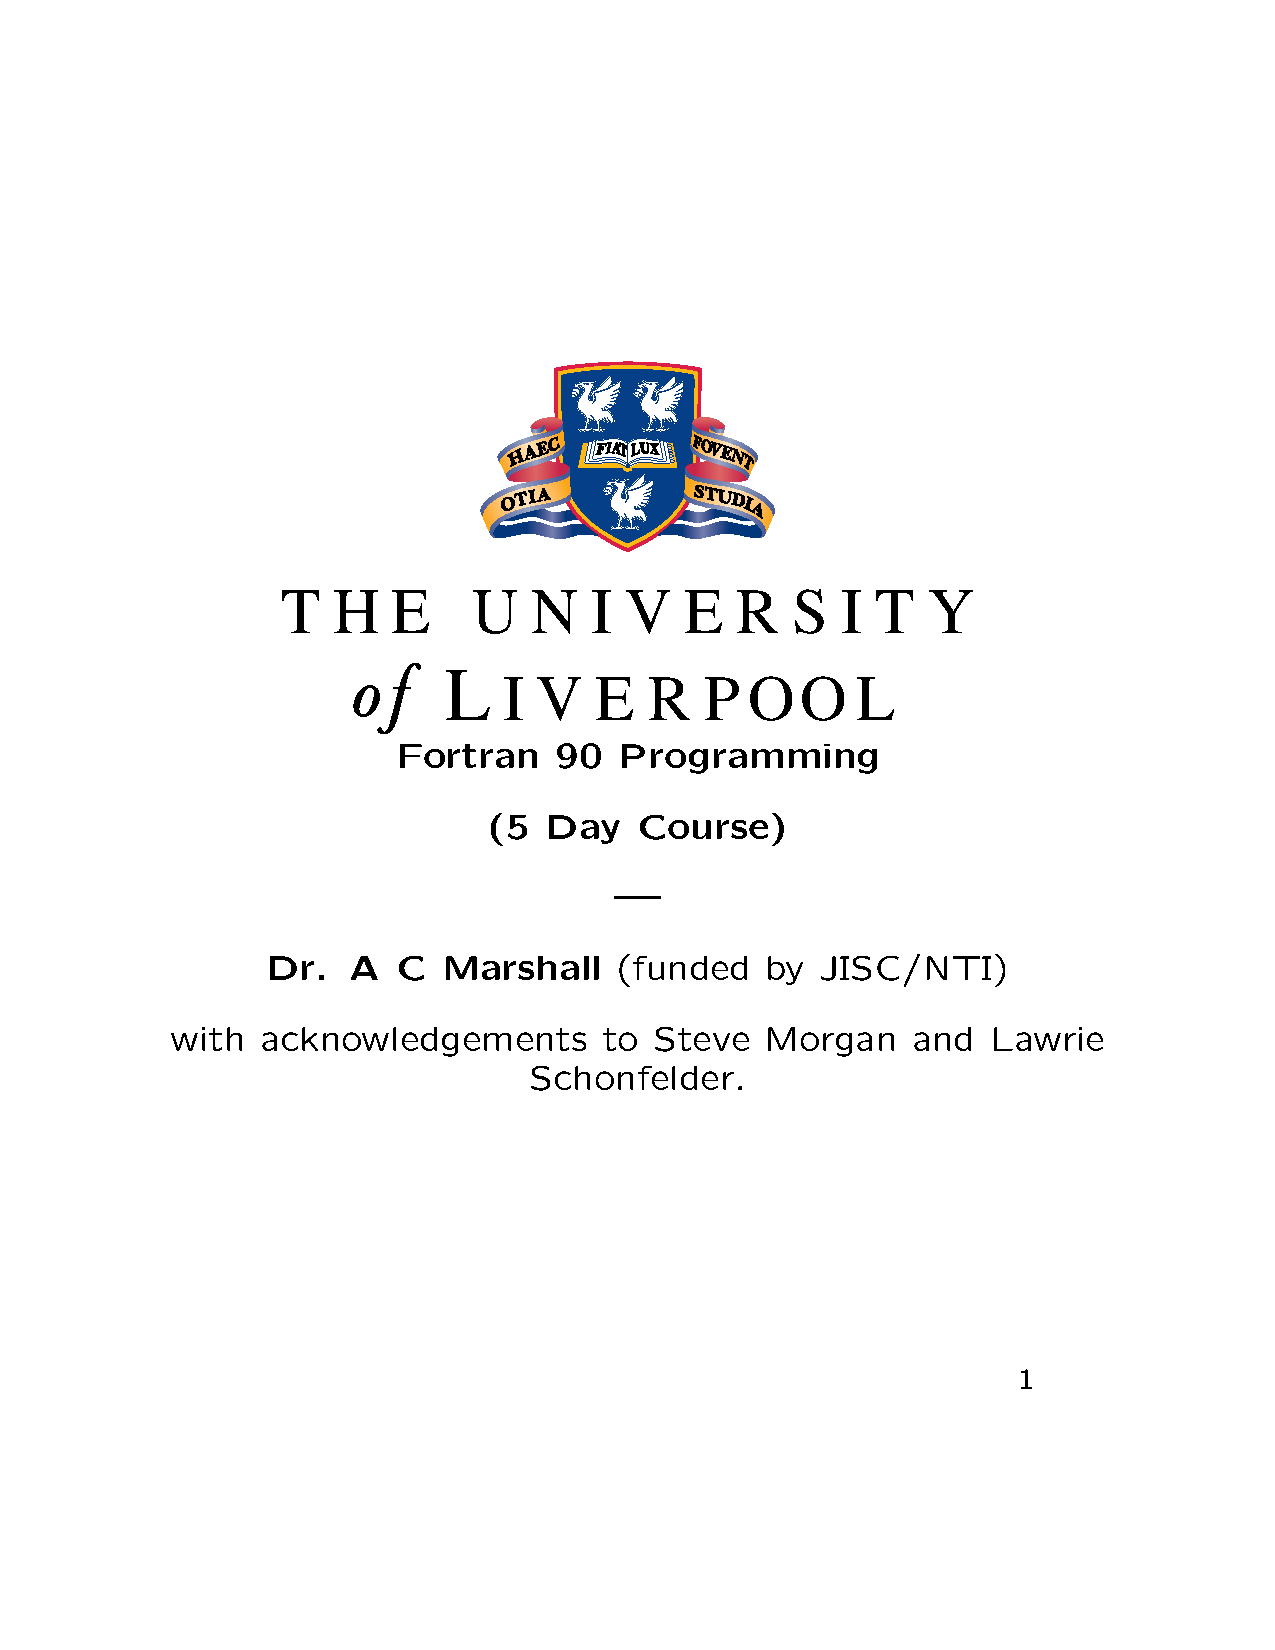
\includepdf[frame=true,scale=0.98,pages={1,3,6-8,10-13,15-21,23-36,38-39,41-54}]{graphics/CourseSlides_clase1.pdf}

\Level 0 {Basic Fortran exercises}
\label{sec:basic-fortran-exercises}

If you have never used Fortran before, the way to run Fortran code is by writing
the ``source'' code in a text file (using any text editor), then compiling the
code, and then executing it.

For example, you could write the following source code in any text editor and
save it as ``test.f90'':

\begin{verbatim}
$ cat hello.f90
PROGRAM HELLO_WORLD
  IMPLICIT NONE

  INTEGER :: count

  PRINT*, "Hello World x 10"
  DO count=1,10
     PRINT*, "Hello World!", count
  END DO

END PROGRAM HELLO_WORLD
\end{verbatim}

Then, in order to translate that source code into an executable file, you need
to compile it (for example with the Fortran compiler in the GCC suite, using the
command ``gfortran''). Below, the option -o tells the compiler to generate an
executable file with name ``hello.x'':

\begin{verbatim}
$ gfortran -o hello.x hello.f90
\end{verbatim}

Then you would have to execute it by typing the number of the executable file
produced above. The syntax ``./'' will tell your shell that the executable file
is located in the directory where you are running this command.

\begin{verbatim}
$ ./hello
 Hello World x 10
 Hello World!           1
 Hello World!           2
 Hello World!           3
 Hello World!           4
 Hello World!           5
 Hello World!           6
 Hello World!           7
 Hello World!           8
 Hello World!           9
 Hello World!          10
\end{verbatim}

Below there are some exercises to familiarize yourself with the features of
Fortran that we have seen in section \ref{sec:basic-fortran}. If you need more
basic exercises, you could try for example the first 10 problems in the Project
Euler website\footnote{https://projecteuler.net/}.

\Level 1 {Read numbers and print them in reverse order}

Write a program that reads first an integer N, and then N integer numbers, which
should then be printed in reverse order.

\begin{verbatim}
$ ./ex1
 Enter number of data to read:
5
 Enter (in one line)           5 integers
34 56 78 98 45
 The data in reverse order are:
          45          98          78          56          34
\end{verbatim}

\Level 1 {Print all leap years between a two given years}

Write a program that given starting and ending years, prints all leap years
within that period. (A year is a leap year if (divisible by 4 but not by 100) or
(divisible by 400)). See: https://en.wikipedia.org/wiki/Leap\_year

\begin{verbatim}
$ ./ex2
 Enter starting and end years
95 120
 Leap years between years          95 and         120 are:
          96
         104
         108
         112
         116
         120
\end{verbatim}

\Level 1 {Write a naïve program to perform matrix multiplication}

This program will expect to first read (using the basic READ* Fortran command) three integers: m,n,p
Then the first matrix (size m x n) will be read row by row.
Then the second matrix (size n x p) will be read row by row.

In order to not type these every time you want to execute the code, we can use
input redirection, which means that we will store in a file the values that we would
normally type in the keyboard. For example, we can have the following file:

\begin{verbatim}
$ cat ex3.input
3 4 5     !! m,n,p
4 5 6 7   !! matriz A (m x n)
8 4 3 2
9 2 4 5
2 5 6 7 8 !! matriz B (n x p)
3 4 1 9 4
8 3 6 4 2
9 6 3 7 1
\end{verbatim}

And then execute the code as follows:

\begin{verbatim}
$ ./ex3 < ex3.input
   134.000000       100.000000       86.0000000       146.000000       71.0000000    
   70.0000000       77.0000000       76.0000000       118.000000       88.0000000    
   101.000000       95.0000000       95.0000000       132.000000       93.0000000
\end{verbatim}

\Level 1 {Write a program that given an integer, checks whether it is
  palindromic (i.e. that can be read the same way backwards and forwards)}

\begin{verbatim}
$ ./ex4
 Enter num
243
 NOT Palindromic

$ ./ex4
 Enter num
5678765
 Palindromic
\end{verbatim}

\Level 1 {Summation Example}
% This example was inspired from
% http://grdelin.phy.hr/~ivo/Nastava/Numericke_metode/literatura/University_of_Liverpool/HTMLF90CourseQuestionsnode59.html

Write a program that given an array of N floats and a W (width), find which W
consecutive numbers have the greatest sum:

\begin{verbatim}
$ cat ex5.input
20   ! N - number of floats
5    ! W - window width
6.3  ! N floats to follow
7.6 
9.2 
3.4 
5.6 
7.23 
9.76 
6.83 
5.45 
4.56
4.86 
5.8 
6.4 
7.43 
7.87 
8.6 
9.25 
8.9 
8.4 
7.23

$ ./ex5 < ex5.input
 Greatest sum is:   43.0200043     given by the following numbers:
   7.86999989    
   8.60000038    
   9.25000000    
   8.89999962    
   8.39999962    
\end{verbatim}

\Level 1 {Salaries Example}
% inspired by
% http://grdelin.phy.hr/~ivo/Nastava/Numericke_metode/literatura/University_of_Liverpool/HTMLF90CourseQuestionsnode61.html

Write a program to calculate the cost to a company of increasing the salary of
its employees. The input will be given as per the following example:

\begin{verbatim}
$ cat ex6.input
9     ! n - number of employees
3     ! nc - number of categories
10500 ! salaries of each employee (n lines)
16140
22300
15960
14150
12180
13230
15760
31000
1     ! category of each employee (n lines)
2
3
2
1
1
1
2
3
5     ! increase (percentage) for each category
4
2

$ ./ex6 < ex6.input
 Current cost:   151220.000      New cost:   156703.406     Difference:   5483.40625    
\end{verbatim}


\Level 1 {Travelling Salesman Problem}
% inspired by
% http://grdelin.phy.hr/~ivo/Nastava/Numericke_metode/literatura/University_of_Liverpool/HTMLF90CourseQuestionsnode63.html

The travelling salesman problem is a very well known and computationally very
hard problem, so this will only work for a very small number of towns, but the
idea is that a salesman travels between a number of towns whose distances
(integer numbers) are given, and you are required to find the shortest route
which brings the salesman to all the towns. Since we haven't seen recursion yet,
the number of towns will be fixed for the time being to 5. Later on we will
improve this to work with any number of towns.

\begin{verbatim}
$ cat ex7.input
5                      ! n - number of towns
0   120 180 202 300    ! n lines, each line indicating the distances from town i [1:5]
120 0   175 340 404    !          to all towns j [1:5]
180 175 0   98  56
202 340 98  0   168
300 404 56  168 0

$ ./ex7 < ex7.input
 Shortest route travelled is :           1           2           3           5           4
 Distance travelled =          721
\end{verbatim}

\Level 1 {N-body problem}

Given the description of the N-body problem in chapter \ref{ch:nbody.tex}, write
a program to solve the N-body problem.




